
\section{Nonlinear normal modes}
\label{sec:nonl-norm-modes}

This is brief introduction to nonlinear normal modes(NNMs). NNMs are considered
an extension to linear normal modes(LNM), but without the mathematical
properties of LNMs. Where LNMs decouple eoms, ie. a solution can be written as a
linear combinations of LNMs, and are invariant, this is not the case for NNMs.

Instead NNMs are defined as \textit{(non-necessarily) synchronous periodic
  motion of the system}~\autocite{kerschen2009a} and computed for the undamped
and unforced system, ie. the hamiltonian system.
Synchronous means that all parts of a system reaches their extreme values and
passes through zero at the same time, ie. vibration in unison. In the case of
internal resonance, where one part vibrates at a integer number of another parts
frequency, the vibration can still be periodic but it is no longer in unison.
This which is why the original definition of NNMs as strict synchronous motion
by Rosenberg in 1966~\autocite{rosenberg1966a} was relaxed to the current
formulation by Kerchen. Thus today, NNMs are simply periodic oscillations of a
conservative system.

NNM have the following properties/features
\begin{itemize}
\item \textit{Frequency-energy dependence}:\\
  Nonlinear systems shows a frequency-energy dependence of their oscillations,
  eg. through hardening or softening behaviour. NNMs plotted in a
  frequency-energy plot show this dependency.
\item \textit{Internal resonances}:\\
  NNMs at well-separated fundamental frequencies may interacts and exchange
  energy.

  To expand a bit: At low energies these modes may have incommensurate natural
  frequencies and do not satisfy internal resonance conditions. Due to the
  energy dependence of their frequencies, however, at higher energies the same
  NNMs may become internally resonant, as their energy-dependent frequencies may
  become commensurate, giving strong nonlinear modal interactions
\item \textit{Traces the lotus of NFRCs}:\\
  For structures with low damping, the NNM backbone traces the locus of the
  resonance peaks.
\end{itemize}
where the energy of the system is the sum of the potential and kinetic energy.

The periodic motion of different NNMs of the same system, might include a
different number of harmonics, ie. there is a nonlinear relationship between the
coordinates during the periodic motion.
This can be seen from the configuration space (ie. a plot of $x_1$ vs. $x_2$ for a
2dof example) where the modal line will either be a straight line, as is the
case for LNMs, or a curve when different harmonics are present where the shape
of the curve depends on the energy of the system.

The latter is the generic case and termed \textit{nonsimilar} NNMs. When special
spatial symmetries exist, the NNMs may degenerate into (energy-invariant)
straight modal line even if the system is nonlinear, termed \textit{similar}
NNMs. An example of the latter is given in section \ref{sec:nnm_similar}.

A more in-depth investigation and history of NNMs can be found
in \autocite{kerschen2009a} and the monograph \autocite[chap 2.]{vakakis2008a}.



\subsection{Example}
\label{sec:nnm_example}

To exemplify some of the fundamental properties of NNMs, the undamped and
unforced 2dof system shown in fig. \ref{fig:nnm_2dof} is used.

\begin{figure}[!ht]
  \centering
  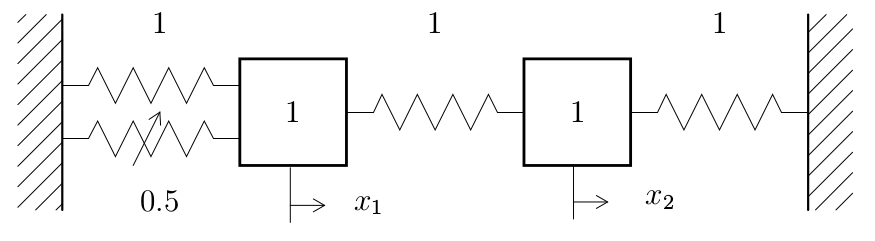
\includegraphics[width=0.7\textwidth]{nnm/2dof_system}
  \caption{Schematic representation of the 2DOF system}
  \label{fig:nnm_2dof}
\end{figure}
where the equations of motion are

\begin{equation}
  \label{eq:nnm_2dof}
  \begin{aligned}
    \ddot x_1 + (2x_1 - x_2) + 0.5 x_1^3 &= 0 \\
    \ddot x_2 + (2x_2 - x_2) &= 0
  \end{aligned}
\end{equation}

This system is said to have an in-phase and out-of-phase mode.
The method for calculating NNMs is given later in section
\ref{sec:shooting_method}.

\subsubsection{Frequency-energy dependence}

As already stated, nonlinear systems have a frequency-energy dependence of their
oscillations. As a consequence the FRF is not invariant. For NNMs, the modal
curves and frequencies also depends on the energy.
NNMs are often represented in a frequency-energy plot (FEP), where a NNM is
represented by a family of points, drawn at the minimal period of the periodic
motion and at an energy equal to the conserved total energy during the motion. A
branch, represented by a solid line, is a family of NNM motions possessing the
same qualitative features (eg. the in-phase NNM motions of a 2dof system).

The The FEP of the 2dof system \eqref{eq:nnm_2dof} is shown in fig
\ref{fig:nnm_fep}. The backbone of the plot is formed by two branches, which
represent in-phase (bottom) and out-of-phase (top) synchronous NNMs. The FEP
shows that nonlinear modal parameters depend on vibrational energy:

\begin{itemize}
\item The frequency(ie. the minimal period), of both the in-phase and
  out-of-phase NNMs increases with the energy level, due to the hardening
  characteristic of the system.
\item The modal curves, ie. the curve drawn in the configuration space defined
  by the displacements $x_1$ and $x_2$, change for increasing energies. They are
  seen in the insets. As energy increases, the straight line becomes curved as a
  sign of the nonlinear relationship which exists between $x_1$ and $x_2$.
\item Although the energy is shared between the two dofs at low-energy, the NNMs
  localise to either dof for increasing energies. The in-phase NNM localise to
  the second dof, whereas the out-of-phase NNM localizes to the first dof, as
  seen by the shape of the modal curve.
\end{itemize}

\begin{figure}[!ht]
  \centering
  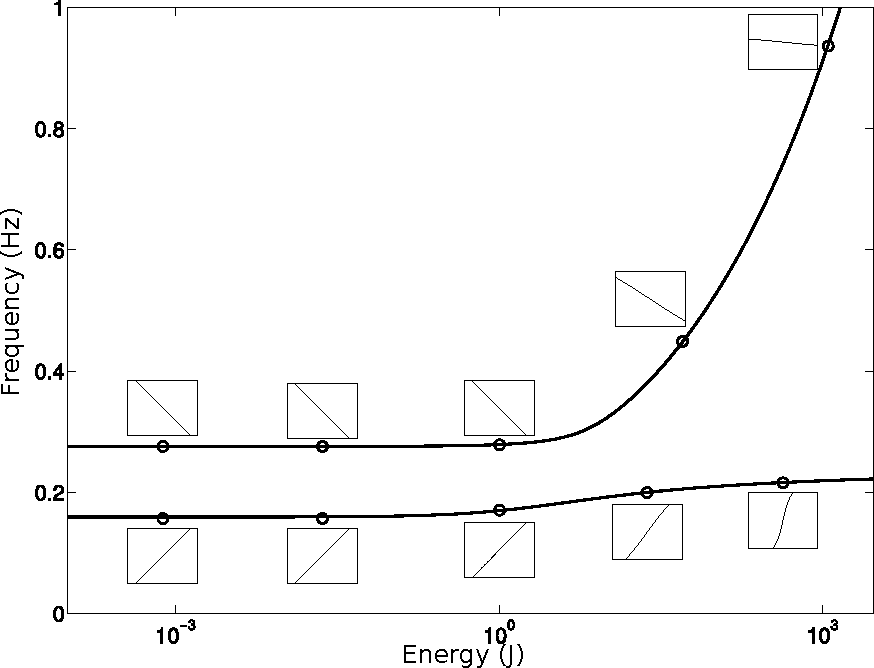
\includegraphics[width=0.7\textwidth]{nnm/2dof_nnm.pdf}
  \caption{Frequency-energy plot of the 2dof system \eqref{eq:nnm_2dof}.
    NNM motions depicted in the configuration space are shown in inserts.
    The aspect ratio of the inserts are equal, used to indicate whether or
    not the motion is localised to a particular dof.}
  \label{fig:nnm_fep}
\end{figure}


\subsubsection{Modal interactions through resonance}

The ratio between the linear natural frequencies of the 2dof system
\eqref{eq:nnm_2dof} is $\sqrt{3}$ as seen in table \ref{tab:nnm_2dof}. Thus they
are not commensurate(ie. $\frac{\omega_1}{\omega_2}$ is not a rational number),
and internal resonance should not occur between the modes.

But due to the frequency-energy dependence and that the frequency of the
in-phase NNM increases less rapidly than that of the out-of-phase, a 3:1 ratio
between the two (mode) frequencies can still be realised. This is seen in the
FEP fig. \ref{fig:nnm_fep_resonance}, where a new branch of periodic solutions
emerges from the in-phase backbone, termed a tongue, and enlarged at the insert.
The dashed line is the out-of-phase backbone shown at one-third of its
frequency, and the point it intersect is the point of internal 3:1 resonance.

\begin{figure}[!ht]
  \centering
  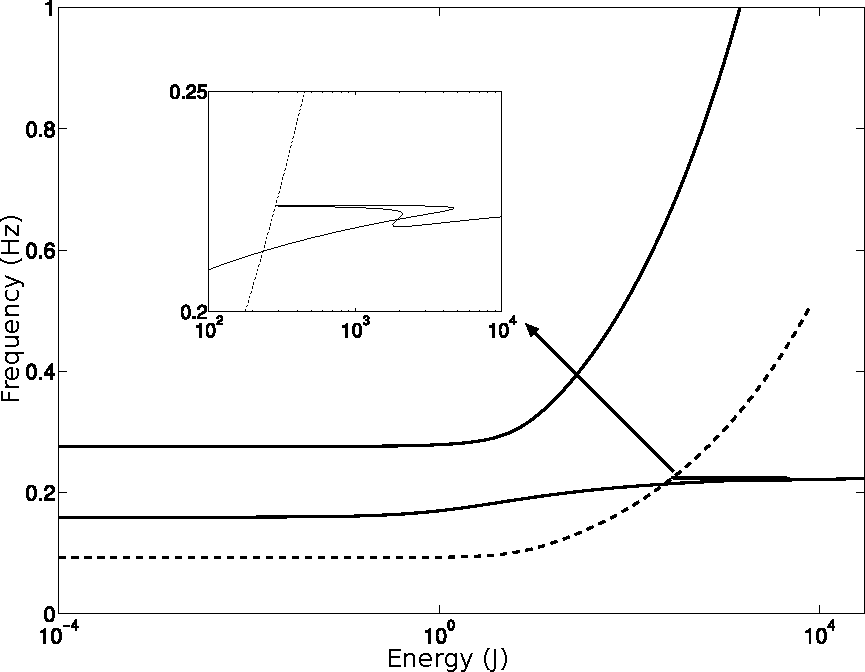
\includegraphics[width=0.7\textwidth]{nnm//2dof_nnm_resonans.pdf}
  \caption{FEP of the 2dof system \eqref{eq:nnm_2dof}. The tongue shows a 3:1
    internal resonance between the in-phase and out-of-phase NNMs.
    \sampleline{dashed}: out-of-phase backbone at one-third of its frequency}
  \label{fig:nnm_fep_resonance}
\end{figure}


The frequency of the out-of-phase NNM increases unbounded for increasing
energies, whereas the in-phase NNM asymptotically approaches $\sqrt{3}$. From
this follows that there, in the formulated framework of NNMs, are a infinity of
internal resonance, ie. 3:1, 4:1, 5:1, etc. Most of these are of course very
hard to realise due to stability and the very large energies(ie. very large
displacements) needed.


Figure \ref{fig:nnm_3:1_resonance} shows the 3:1 resonance. The motion is still
periodic, but not in unison.

\begin{figure}[!ht]
  \centering
  \begin{subfigure}[b]{0.45\textwidth}
    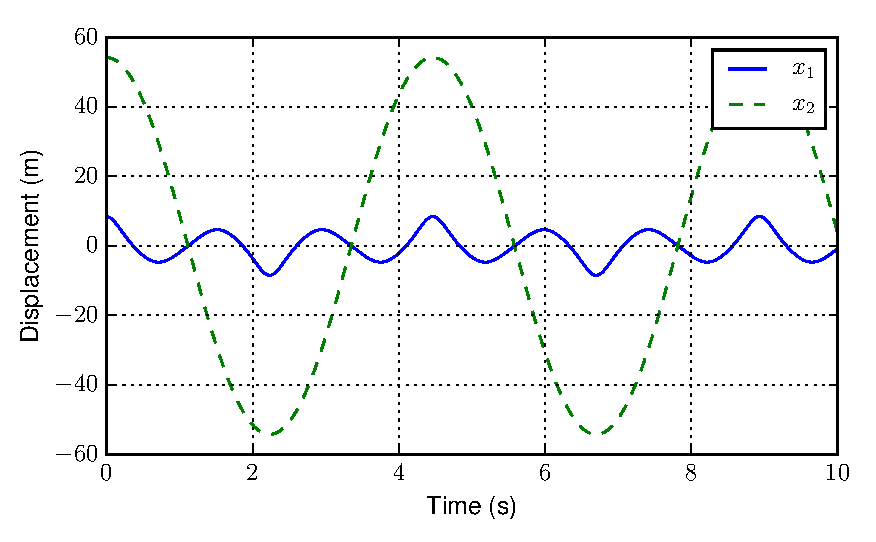
\includegraphics[width=\textwidth]{nnm/nonlin_31_time_hist}
  \end{subfigure}
  ~
  \begin{subfigure}[b]{0.45\textwidth}
    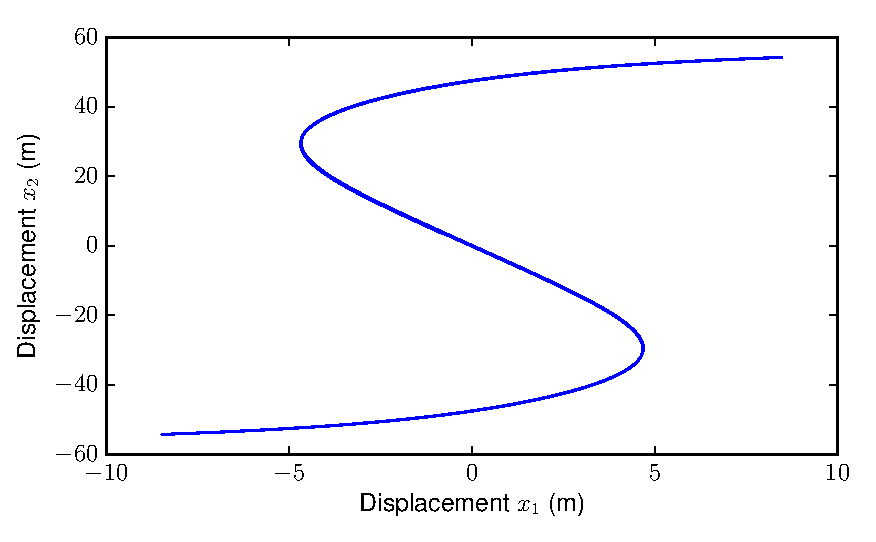
\includegraphics[width=\textwidth]{nnm/nonlin_31_conf_space}
  \end{subfigure}
  \caption{Internally 3:1 resonant NNMs of the 2dof system \eqref{eq:nnm_2dof}.
    $[x_1, x_2, \dot x_1, \dot x_2] = [8.476, 54.263, 0, 0]$;
    \textbf{(a)}: time series;
    \textbf{(b)}: configuration space}
  \label{fig:nnm_3:1_resonance}
\end{figure}


\subsubsection{Mode bifurcation and stability}
\label{sec:nnm_similar}

A third property of NNMs is that their number may exceed the number of DOFs, and
thus LNMs, of the system. Due to mode bifurcations, not all NNMs can be regarded
as extensions of LNMs. An example of NNM bifurcation is given by the system
\autocite{vakakis1992a}

\begin{equation}
   \label{eq:nnm_similar_sys}
   \begin{aligned}
     \ddot x_1 + k_3(x_1 - x_2)^3 + x_1 + x_1^3&= 0 \\
     \ddot x_2 - k_3(x_2 - x_2)^3 + x_2 + x_2^3&= 0
   \end{aligned}
\end{equation}
where $k_3$ is the strength of the nonlinear coupling. Note that this system is
symmetric and thus only possesses \textit{similar} NNMs having the relation $x_2
= c x_1$, where $c$ is a real modal constant.

Insert the relation in eq. \ref{eq:nnm_similar_sys} to eliminate $x_2$
\begin{equation}
   \label{eq:nnm_similar_sys2}
   \begin{aligned}
     \ddot x_1 + x_1 + \left(1 + k_3(1-c)^3 \right)x_1^3 &= 0 \\
     \ddot x_1 + x_1 - \frac{1}{c} \left(c^3 + k_3(1-c)^3 \right)x_1^3 &= 0
   \end{aligned}
\end{equation}

As both equations satisfy the same solution, the modal constant satisfy
\begin{equation}
  \label{eq:nmm_similar_modal}
  k_3(1+c)(c-1)^3 = c(1-c^2), \quad c \neq 0
\end{equation}

From this, it follows that the system \ref{eq:nnm_similar_sys} always have two
modes characterised by $c\pm1$, the in- and out-of-phase motion respectively, which
is a direct extension of LNM. However there is also the solution
\begin{equation}
  c\neq 1, \quad k = - \frac{c}{(c-1)^2}
\end{equation}
as shown in fig \ref{fig:nnm_similar_bifur}. At $k_3 = 0.25$ the
out-of-phase NNM bifurcates into two additional similar NNMs and become
unstable. Unstable NNMs are not physical realisable, as small perturbations of
the initial conditions that generate said NNM motion lead to the elimination of
the mode oscillation.


\begin{figure}[!ht]
  \centering
  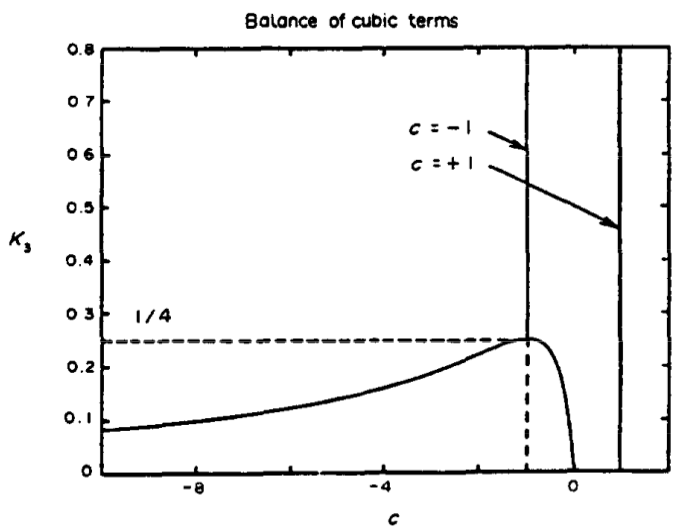
\includegraphics[width=0.7\textwidth]{nnm/similar-nnm-bifur}
  \caption{Pitchfork bifurcation of NMMs; the solution of eq
    \eqref{eq:nmm_similar_modal}. (---) stable mode, (- - -) unstable mode.
    Copied from \autocite{vakakis1992a}}
  \label{fig:nnm_similar_bifur}
\end{figure}


Figure \ref{fig:nnm_similar} shows the time series and corresponding
configuration space for the ``bifurcated'' out-of-phase NNM for
\eqref{eq:nnm_similar_sys}. The system still vibrates with a single harmonic in
unison, as seen by the straight line in configuration space and the time series;
as expected for similar systems.

\begin{figure}[!ht]
  \centering
  \begin{subfigure}[b]{0.45\textwidth}
    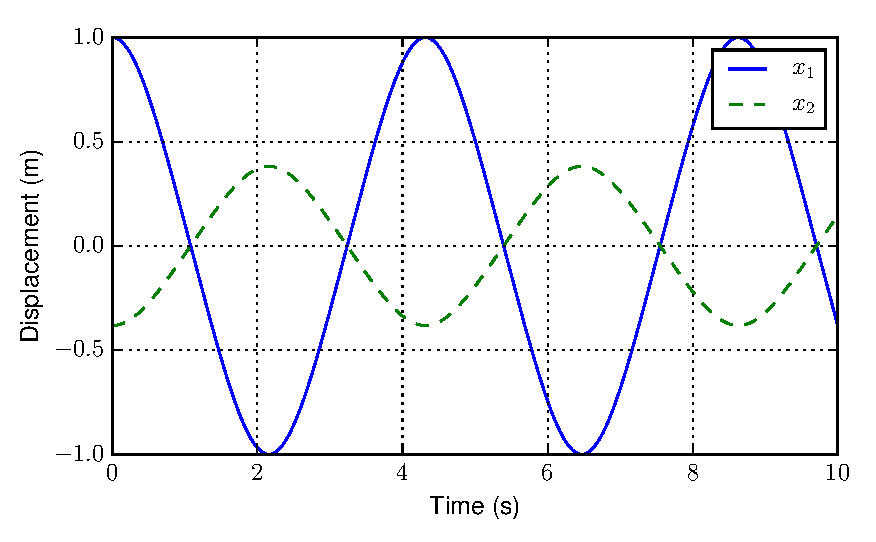
\includegraphics[width=\textwidth]{nnm/similar1_time_hist}
  \end{subfigure}
  ~
  \begin{subfigure}[b]{0.45\textwidth}
    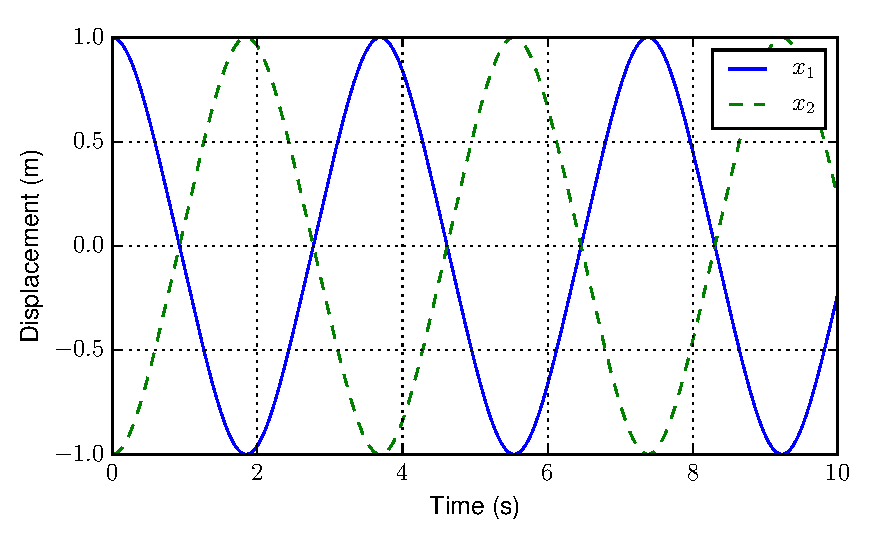
\includegraphics[width=\textwidth]{nnm/similar2_time_hist}
  \end{subfigure} \\
  \begin{subfigure}[b]{0.45\textwidth}
    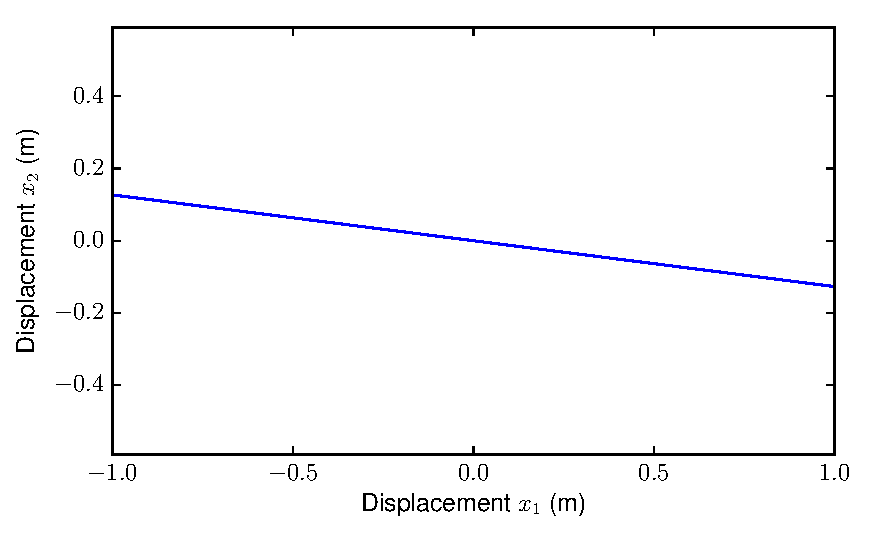
\includegraphics[width=\textwidth]{nnm/similar1_conf_space}
  \end{subfigure}
  ~
  \begin{subfigure}[b]{0.45\textwidth}
    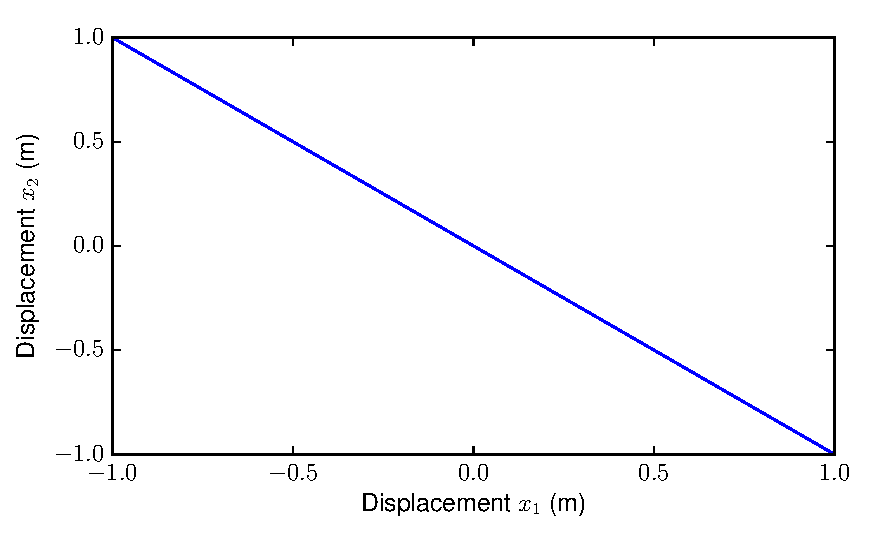
\includegraphics[width=\textwidth]{nnm/similar2_conf_space}
  \end{subfigure}
  \caption{Time series and corresponding configuration space for the
    ``bifurcated'' out-of-phase NNM, system \eqref{eq:nnm_similar_sys} with
    $k_3=0.2$.
    \textbf{(left)}: $[x_1, x_2, \dot x_1, \dot x_2] = [1,-1,0,0]$;
    \textbf{(right)}: $[x_1, x_2, \dot x_1, \dot x_2] = [1, -0.3820,0,0]$.}
  \label{fig:nnm_similar}
\end{figure}






% Figure \ref{fig:nonlin_time_series} and \ref{fig:nonlin_nnm_config} shows the
% time series and configuration plane for in-phase and out-of-phase NNMs for the
% nonlinear system. The system vibrates in unison, even though higher harmonics
% are present as seen by the curved modal lines in the configuration plot.


% \begin{figure}[!ht]
%   \centering
%   \begin{subfigure}[b]{0.45\textwidth}
%     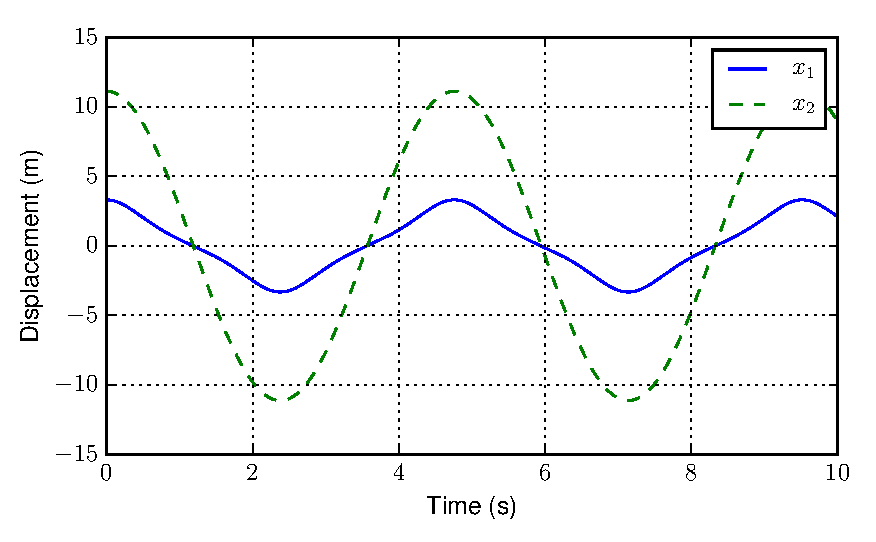
\includegraphics[width=\textwidth]{nnm/nonlin_inphase_time_hist}
%   \end{subfigure}
%   ~
%   \begin{subfigure}[b]{0.45\textwidth}
%     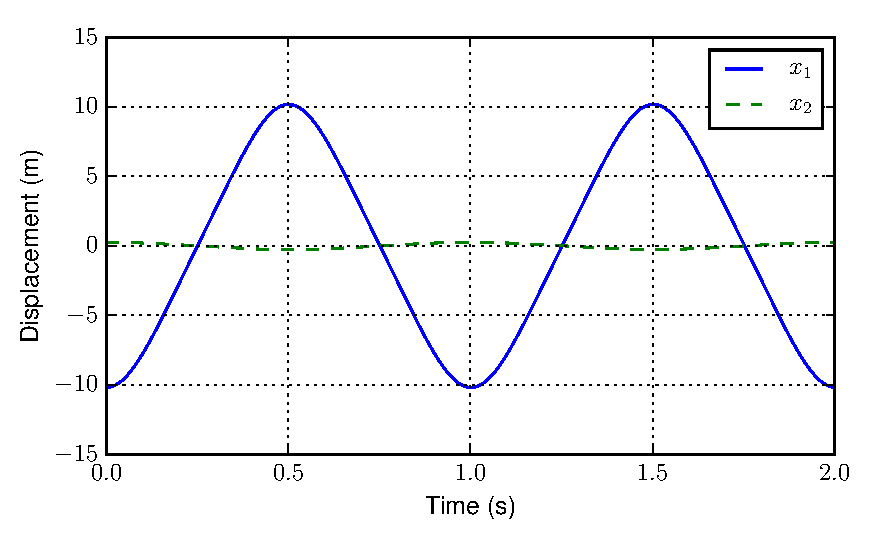
\includegraphics[width=\textwidth]{nnm/nonlin_outphase_time_hist}
%   \end{subfigure}
%   \caption{Time series of system (\ref{eq:2dof_nonlin_sys}).
%     Left plot: in-phase NNM,
%     $[x_1(0), x_2(0), \dot x_1(0), \dot x_2(0)] = [3.319, 11.134,0,0]$;
%     Right plot: out-of-phase NNM,
%     $[x_1(0), x_2(0), \dot x_1(0), \dot x_2(0)] = [-10.188, 0.262,0,0]$.}
%   \label{fig:nonlin_time_series}
% \end{figure}

% \begin{figure}[!ht]
%   \centering
%   \begin{subfigure}[b]{0.45\textwidth}
%     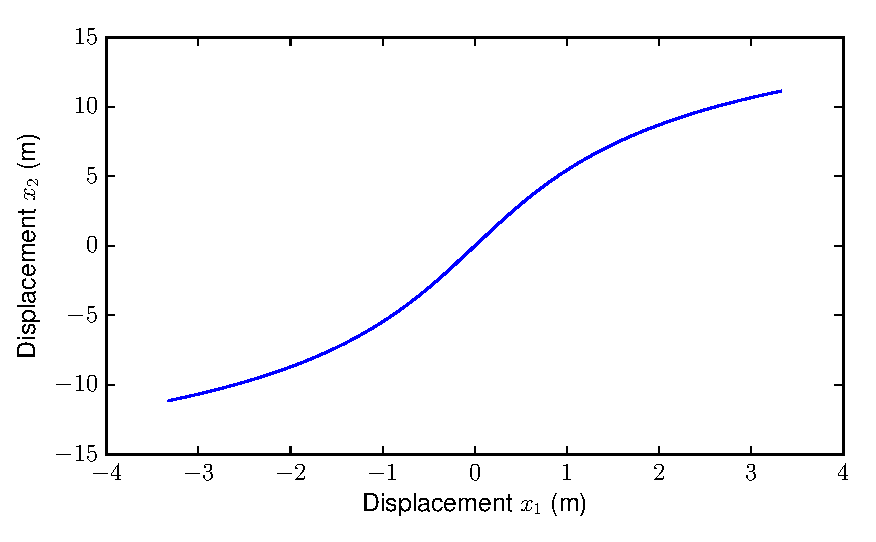
\includegraphics[width=\textwidth]{nnm/nonlin_inphase_conf_space}
%   \end{subfigure}
%   ~
%   \begin{subfigure}[b]{0.45\textwidth}
%     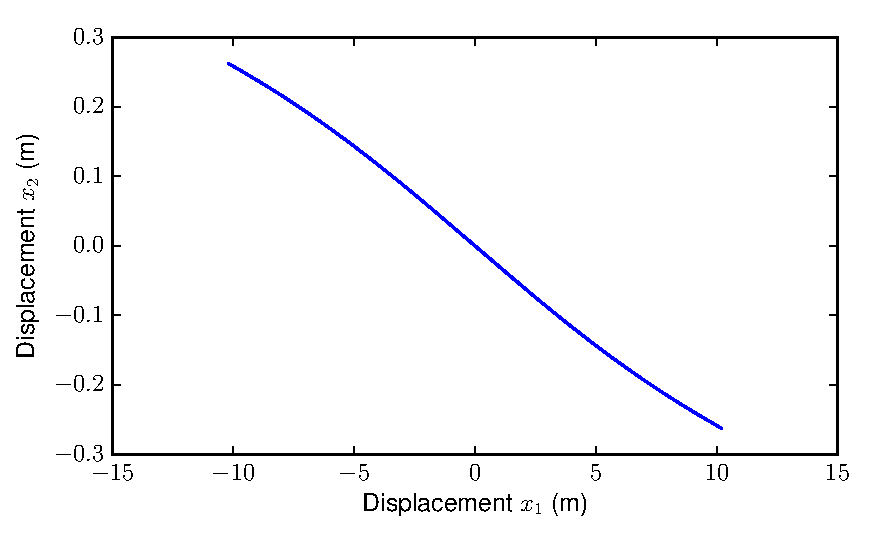
\includegraphics[width=\textwidth]{nnm/nonlin_outphase_conf_space}
%   \end{subfigure}
%   \caption{NNM motion of system (\ref{eq:2dof_nonlin_sys}) in configuration space.
%     Left plot: in-phase NNM;
%     Right plot: of-phase NNM.}
%   \label{fig:nonlin_nnm_config}
% \end{figure}


\subsection{Summary}

NNMs are merely a periodic solution of the eom. Contrary to LNMs, NNMs might
become unstable through bifurcations and their numbers might exceed the number
of DOFs. Neither are they invariant, as NNMs shows a frequency-energy
dependency.

Thus, even if they do not have the mathematical properties of LNMs, ie.NNMs are
not orthogonal, cannot decouple eoms and cannot be superposed to calculate the
response, they are still useful for understanding some nonlinear phenomenons of
lightly damped systems (NNMs are calculated for the underlying
Hamiltonian(undamped and unforced) structure)

\begin{itemize}
\item Modal interactions, where frequency-energy dependence result in internal
  resonance.
\item Trace the lotus of a nonlinear system for various energies, ie. the
  resonance.
\end{itemize}


%%% Local Variables:
%%% mode: latex
%%% TeX-master: "../../report"
%%% End:
